\documentclass[12pt,a4paper]{report}
\usepackage[utf-8]{inputenc}
\usepackage[english]{babel}
\usepackage[margin=1in]{geometry}
\usepackage{graphicx}
\usepackage{tikz}
\usepackage{hyperref}
\usepackage{listings}
\usepackage{xcolor}
\usepackage{fancyhdr}
\usepackage{lastpage}
\usepackage{caption}
\usepackage{subcaption}
\usepackage{booktabs}
\usepackage{array}

% Code listing style
\lstset{
    language=python,
    basicstyle=\ttfamily\small,
    keywordstyle=\color{blue},
    commentstyle=\color{gray},
    stringstyle=\color{red},
    breaklines=true,
    showstringspaces=false,
    tabsize=4,
    frame=single,
    backgroundcolor=\color{lightgray!20}
}

% Header and footer
\pagestyle{fancy}
\fancyhf{}
\rhead{Card Signal Board}
\lhead{DevOps Project Report}
\cfoot{Page \thepage\ of \pageref{LastPage}}

% TikZ libraries
\usetikzlibrary{shapes,arrows,positioning,shadows,shapes.geometric}

\title{\textbf{Card Signal Board API}\\
       \large A Complete DevOps Project: From Development to Kubernetes Deployment}
\author{Mohamed Bouafif}
\date{\today}

\begin{document}

\maketitle

\tableofcontents
\newpage

\chapter{Executive Summary}

This report documents a comprehensive DevOps engineering project where a FastAPI-based microservice was developed, containerized, deployed to Kubernetes, and automated with CI/CD pipelines. The project demonstrates professional software engineering practices including version control, code review, automated testing, security scanning, containerization, orchestration, and infrastructure as code.

\textbf{Key Achievements:}
\begin{itemize}
    \item Built a complete FastAPI REST API with 6 endpoints and observability features
    \item Implemented 14 comprehensive unit tests with 100\% endpoint coverage
    \item Created production-ready Docker containers with multi-stage builds
    \item Set up automated CI/CD pipeline with testing, security scanning, and Docker builds
    \item Deployed to Kubernetes with 3 replicas, health checks, and auto-scaling
    \item Created parameterized Helm charts for environment-specific deployments
    \item Merged 7 professional pull requests following DevOps best practices
\end{itemize}

\chapter{Project Overview}

\section{Objectives}

The primary objective was to build a small backend service and practice DevOps concepts end-to-end, including:
\begin{enumerate}
    \item Backend API development with modern frameworks
    \item Containerization with Docker
    \item Kubernetes orchestration
    \item CI/CD automation
    \item Infrastructure as Code (IaC)
    \item Observability (metrics, logging, tracing)
    \item Professional Git workflow with code review
\end{enumerate}

\section{Technology Stack}

\begin{table}[h]
\centering
\begin{tabular}{|p{3cm}|p{4cm}|p{4cm}|}
\hline
\textbf{Layer} & \textbf{Technology} & \textbf{Purpose} \\
\hline
\textbf{Language} & Python 3.10 & Application development \\
\hline
\textbf{Framework} & FastAPI 0.109.0 & REST API development \\
\hline
\textbf{ASGI Server} & Uvicorn 0.27.0 & Application server \\
\hline
\textbf{Data Validation} & Pydantic 2.5.0 & Request/response validation \\
\hline
\textbf{Observability} & Prometheus 0.19.0 & Metrics collection \\
\hline
\textbf{Testing} & pytest 7.4.3 & Unit testing framework \\
\hline
\textbf{Containerization} & Docker & Application containerization \\
\hline
\textbf{Orchestration} & Kubernetes 1.20+ & Container orchestration \\
\hline
\textbf{Package Manager} & Helm 3.0+ & K8s deployment management \\
\hline
\textbf{CI/CD} & GitHub Actions & Automated testing and deployment \\
\hline
\textbf{Code Quality} & Black, flake8, Bandit & Linting and security \\
\hline
\textbf{Vulnerability Scan} & Trivy & Container image scanning \\
\hline
\textbf{Version Control} & Git/GitHub & Source code management \\
\hline
\end{tabular}
\end{table}

\chapter{System Architecture}

\section{Application Architecture}

\begin{figure}[h]
\centering
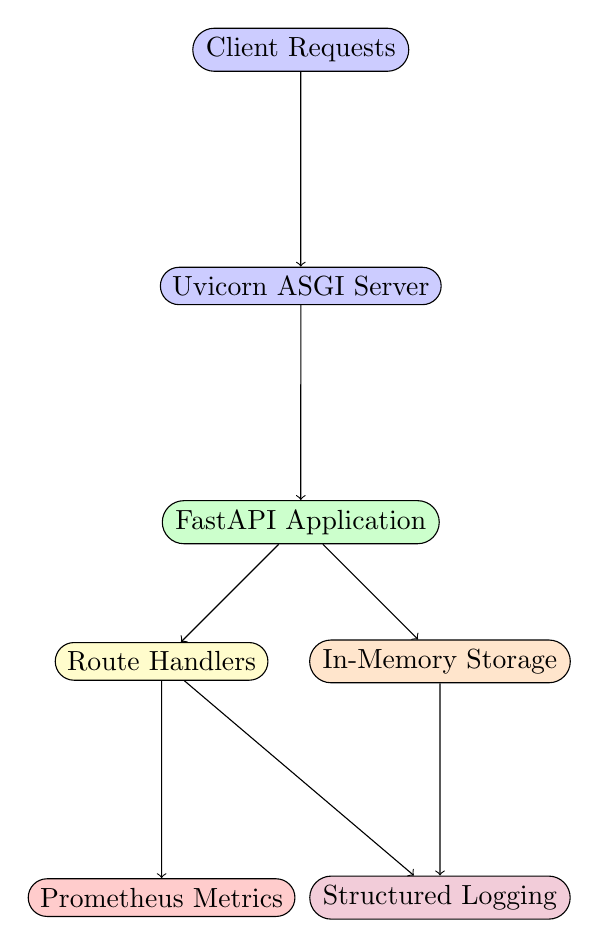
\begin{tikzpicture}[node distance=3cm, every node/.style={draw, rounded rectangle, fill=blue!20}]
    
    \node (client) at (0,3) {Client Requests};
    \node (uvicorn) [below of=client] {Uvicorn ASGI Server};
    \node (fastapi) [below of=uvicorn, fill=green!20] {FastAPI Application};
    \node (routes) [below left of=fastapi, fill=yellow!20, node distance=2.5cm] {Route Handlers};
    \node (db) [below right of=fastapi, fill=orange!20, node distance=2.5cm] {In-Memory Storage};
    \node (metrics) [below of=routes, fill=red!20] {Prometheus Metrics};
    \node (logging) [below of=db, fill=purple!20] {Structured Logging};
    
    \draw[->] (client) -- (uvicorn);
    \draw[->] (uvicorn) -- (fastapi);
    \draw[->] (fastapi) -- (routes);
    \draw[->] (fastapi) -- (db);
    \draw[->] (routes) -- (metrics);
    \draw[->] (routes) -- (logging);
    \draw[->] (db) -- (logging);
\end{tikzpicture}
\caption{Application Architecture}
\end{figure}

The application is built on FastAPI with:
\begin{itemize}
    \item \textbf{6 REST Endpoints:} Create, Read, List, Delete cards + token verification + health checks
    \item \textbf{In-Memory Database:} Dictionary-based storage with 7-day TTL
    \item \textbf{Metrics:} Prometheus metrics for request count and response time
    \item \textbf{Logging:} Structured logging with request tracing
\end{itemize}

\section{Containerization}

\begin{figure}[h]
\centering
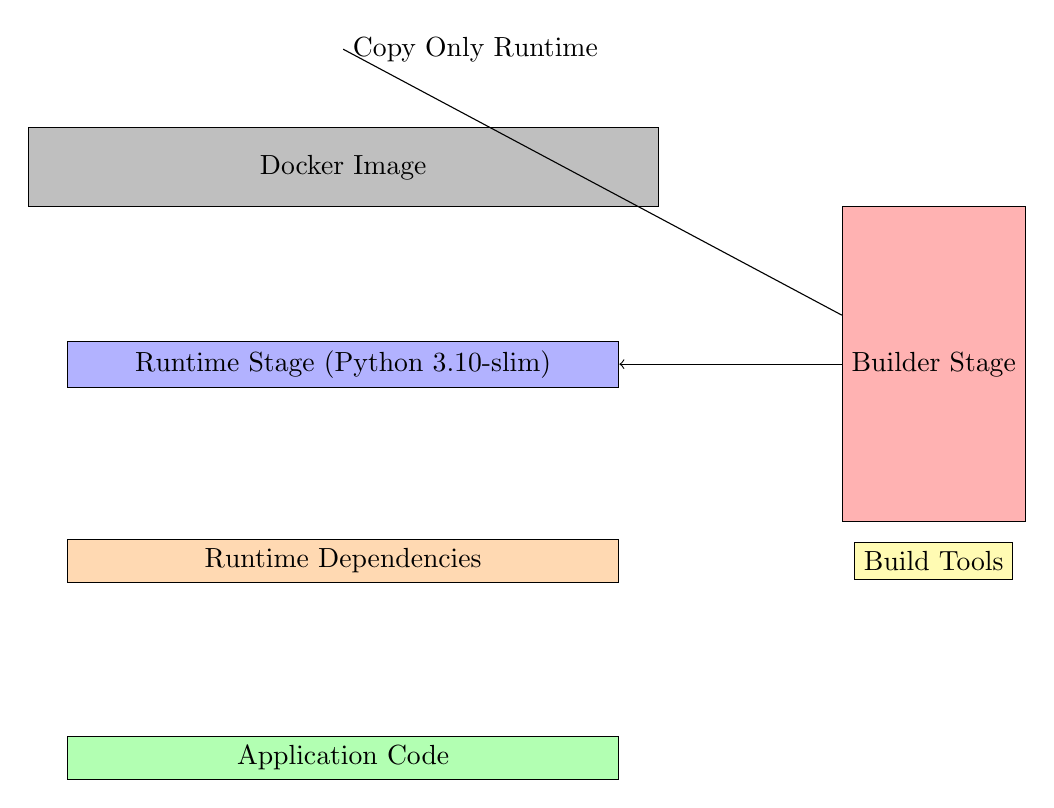
\begin{tikzpicture}[node distance=2.5cm]
    
    % Docker layers
    \node[draw, fill=lightgray, minimum width=8cm, minimum height=1cm] (docker) at (0,0) {Docker Image};
    
    \node[draw, fill=blue!30, below of=docker, minimum width=7cm] (runtime) {Runtime Stage (Python 3.10-slim)};
    \node[draw, fill=orange!30, below of=runtime, minimum width=7cm] (deps) {Runtime Dependencies};
    \node[draw, fill=green!30, below of=deps, minimum width=7cm] (app) {Application Code};
    
    \node[draw, fill=red!30, right of=runtime, xshift=5cm, minimum height=4cm] (builder) {Builder Stage};
    \node[draw, fill=yellow!30, below of=builder] (compile) {Build Tools};
    
    \draw[->] (builder) -- (runtime);
    \draw[right] (builder) -- (0, 1.5) node[right] {Copy Only Runtime};
    
\end{tikzpicture}
\caption{Multi-Stage Docker Build Process}
\end{figure}

Multi-stage Docker build optimizes image size:
\begin{itemize}
    \item \textbf{Builder Stage:} Compiles dependencies
    \item \textbf{Runtime Stage:} Minimal base image with only runtime dependencies
    \item \textbf{Result:} Smaller, more secure image
\end{itemize}

\chapter{CI/CD Pipeline}

\section{Pipeline Overview}

\begin{figure}[h]
\centering
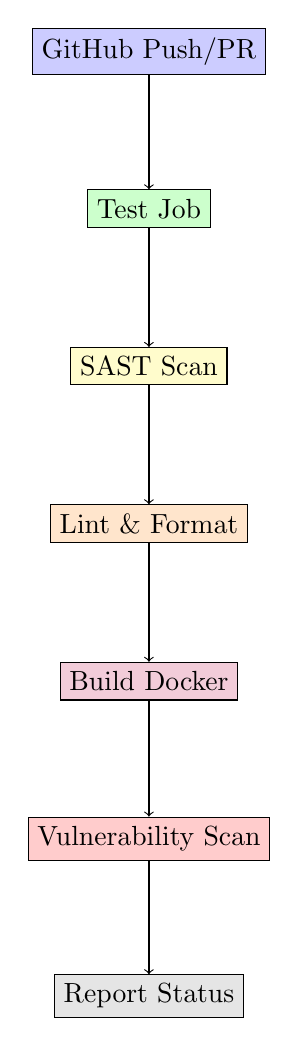
\begin{tikzpicture}[node distance=2cm, every node/.style={draw, rectangle, fill=blue!20}]
    
    \node (trigger) {GitHub Push/PR};
    \node (test) [below of=trigger, fill=green!20] {Test Job};
    \node (sast) [below of=test, fill=yellow!20] {SAST Scan};
    \node (lint) [below of=sast, fill=orange!20] {Lint \& Format};
    \node (build) [below of=lint, fill=purple!20] {Build Docker};
    \node (trivy) [below of=build, fill=red!20] {Vulnerability Scan};
    \node (report) [below of=trivy, fill=gray!20] {Report Status};
    
    \draw[->] (trigger) -- (test);
    \draw[->] (test) -- (sast);
    \draw[->] (sast) -- (lint);
    \draw[->] (lint) -- (build);
    \draw[->] (build) -- (trivy);
    \draw[->] (trivy) -- (report);
    
\end{tikzpicture}
\caption{CI/CD Pipeline Workflow}
\end{figure}

\section{Pipeline Jobs}

\begin{table}[h]
\centering
\begin{tabular}{|p{2cm}|p{3cm}|p{4cm}|}
\hline
\textbf{Job} & \textbf{Tool} & \textbf{Purpose} \\
\hline
Test & pytest + coverage & Unit tests with coverage reporting \\
\hline
SAST & Bandit & Static security analysis \\
\hline
Lint & Black + flake8 & Code quality and formatting \\
\hline
Build & Docker buildx & Container image creation \\
\hline
Security & Trivy & Vulnerability scanning \\
\hline
Report & Bash script & Final pipeline status \\
\hline
\end{tabular}
\end{table}

\section{Workflow Triggers}

The pipeline automatically runs on:
\begin{itemize}
    \item \textbf{Push to main/develop branches:} Full pipeline including build and push
    \item \textbf{Pull Requests:} Test, SAST, lint, and security scans (no push)
    \item \textbf{Manual Trigger:} Via workflow\_dispatch for on-demand runs
\end{itemize}

\chapter{Kubernetes Deployment}

\section{Deployment Architecture}

\begin{figure}[h]
\centering
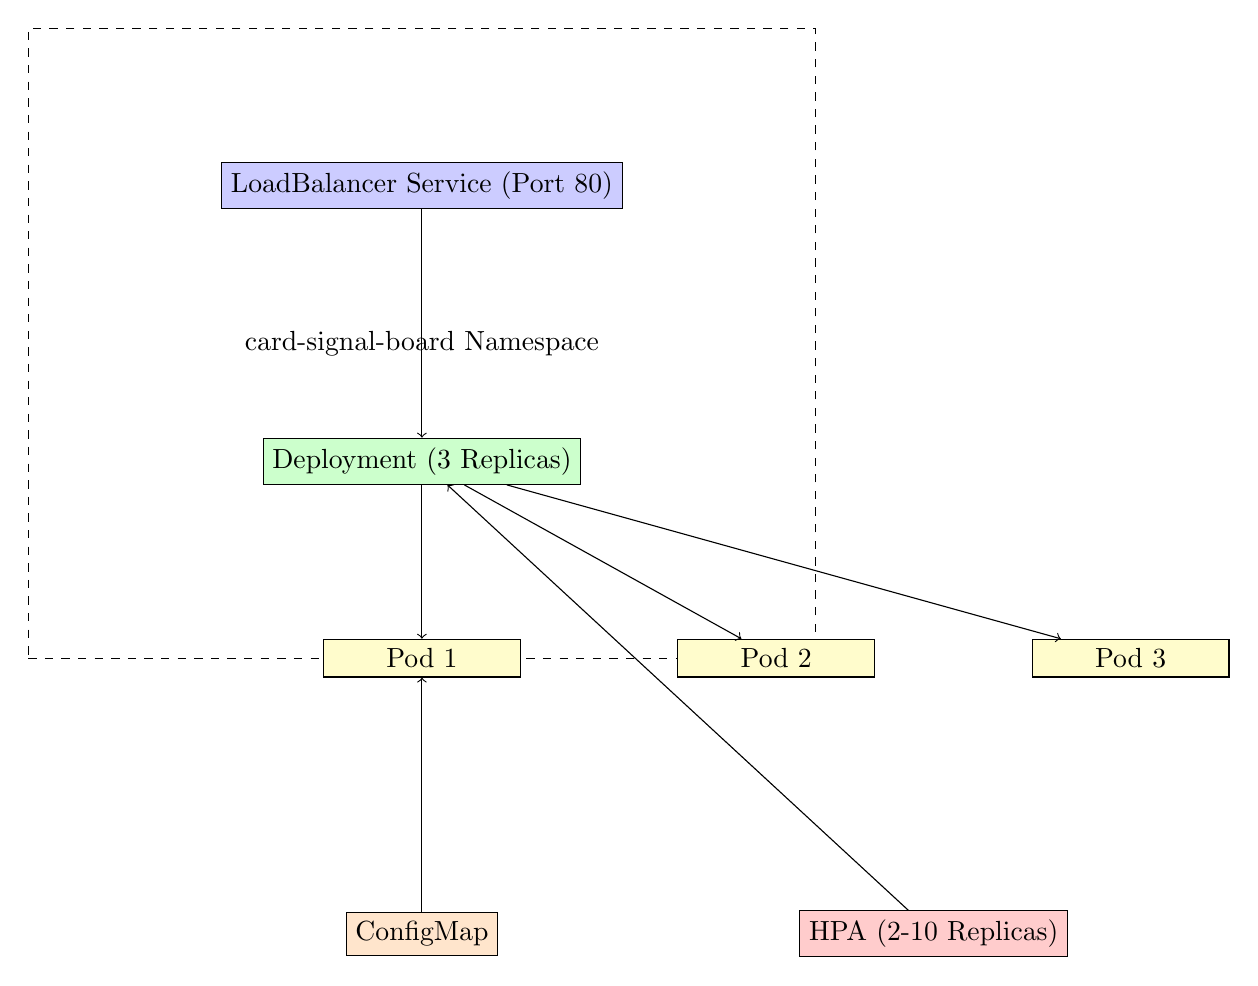
\begin{tikzpicture}[node distance=2.5cm]
    
    % Namespace
    \node[draw, rectangle, dashed, minimum width=10cm, minimum height=8cm] (ns) {card-signal-board Namespace};
    
    % Service
    \node[draw, fill=blue!20, anchor=north, above of=ns, yshift=-0.5cm] (svc) {LoadBalancer Service (Port 80)};
    
    % Deployment
    \node[draw, fill=green!20, below of=svc, yshift=-1cm] (deploy) {Deployment (3 Replicas)};
    
    % Pods
    \node[draw, fill=yellow!20, below of=deploy, minimum width=2.5cm] (pod1) {Pod 1};
    \node[draw, fill=yellow!20, right of=pod1, xshift=2cm, minimum width=2.5cm] (pod2) {Pod 2};
    \node[draw, fill=yellow!20, right of=pod2, xshift=2cm, minimum width=2.5cm] (pod3) {Pod 3};
    
    % ConfigMap and HPA
    \node[draw, fill=orange!20, below of=pod1, yshift=-1cm] (cm) {ConfigMap};
    \node[draw, fill=red!20, right of=cm, xshift=4cm] (hpa) {HPA (2-10 Replicas)};
    
    \draw[->] (svc) -- (deploy);
    \draw[->] (deploy) -- (pod1);
    \draw[->] (deploy) -- (pod2);
    \draw[->] (deploy) -- (pod3);
    \draw[->] (cm) -- (pod1);
    \draw[->] (hpa) -- (deploy);
    
\end{tikzpicture}
\caption{Kubernetes Deployment Architecture}
\end{figure}

\section{Deployment Features}

\begin{table}[h]
\centering
\begin{tabular}{|p{3cm}|p{5cm}|}
\hline
\textbf{Feature} & \textbf{Implementation} \\
\hline
High Availability & 3 replicas with rolling updates \\
\hline
Auto-Scaling & HPA scales 2-10 based on CPU 70\% / Memory 80\% \\
\hline
Health Checks & Liveness (10s) and Readiness (5s) probes \\
\hline
Resource Limits & CPU: 100m-500m, Memory: 64Mi-256Mi \\
\hline
Security & Non-root user, read-only filesystem, dropped capabilities \\
\hline
Configuration & ConfigMap for environment variables \\
\hline
Observability & Prometheus annotations for metrics scraping \\
\hline
Graceful Shutdown & 30-second termination grace period \\
\hline
\end{tabular}
\end{table}

\section{Deployment Commands}

\begin{lstlisting}[language=bash]
# Apply all Kubernetes manifests
kubectl apply -f k8s/

# Verify deployment
kubectl get deployments -n card-signal-board
kubectl get pods -n card-signal-board
kubectl get svc -n card-signal-board

# Check logs
kubectl logs -f -n card-signal-board -l app=card-signal-board
\end{lstlisting}

\chapter{Infrastructure as Code: Helm}

\section{Helm Chart Structure}

\begin{figure}[h]
\centering
\begin{lstlisting}[language=bash]
helm/card-signal-board/
├── Chart.yaml              # Chart metadata
├── values.yaml             # Default configuration
├── templates/
│   ├── _helpers.tpl       # Template helpers
│   ├── namespace.yaml      # Namespace
│   ├── deployment.yaml     # Deployment
│   ├── service.yaml        # Service
│   ├── configmap.yaml      # Configuration
│   ├── hpa.yaml           # Auto-scaling
│   └── serviceaccount.yaml # RBAC
└── README.md              # Documentation
\end{lstlisting}
\caption{Helm Chart Directory Structure}
\end{figure}

\section{Helm Usage Examples}

\begin{lstlisting}[language=bash]
# Install with default values
helm install card-signal-board ./helm/card-signal-board -n csb --create-namespace

# Install with custom values
helm install card-signal-board ./helm/card-signal-board -f values-prod.yaml

# Upgrade deployment
helm upgrade card-signal-board ./helm/card-signal-board --set image.tag=v1.0.0

# Rollback to previous release
helm rollback card-signal-board 1

# Template validation
helm template card-signal-board ./helm/card-signal-board --dry-run

# View release info
helm status card-signal-board -n csb
\end{lstlisting}

\section{Parameterized Configuration}

The Helm chart supports 30+ configurable parameters:

\begin{table}[h]
\centering
\begin{tabular}{|p{3cm}|p{2cm}|p{3cm}|}
\hline
\textbf{Parameter} & \textbf{Default} & \textbf{Description} \\
\hline
replicaCount & 3 & Number of pod replicas \\
\hline
image.repository & card-signal-board & Docker image name \\
\hline
image.tag & latest & Docker image tag \\
\hline
service.type & LoadBalancer & Kubernetes service type \\
\hline
autoscaling.enabled & true & Enable HPA \\
\hline
autoscaling.minReplicas & 2 & Minimum replicas \\
\hline
autoscaling.maxReplicas & 10 & Maximum replicas \\
\hline
resources.limits.cpu & 500m & CPU limit \\
\hline
resources.limits.memory & 256Mi & Memory limit \\
\hline
\end{tabular}
\end{table}

\chapter{Development Workflow}

\section{Git Branching Strategy}

The project followed a professional Git workflow with 7 feature branches:

\begin{figure}[h]
\centering
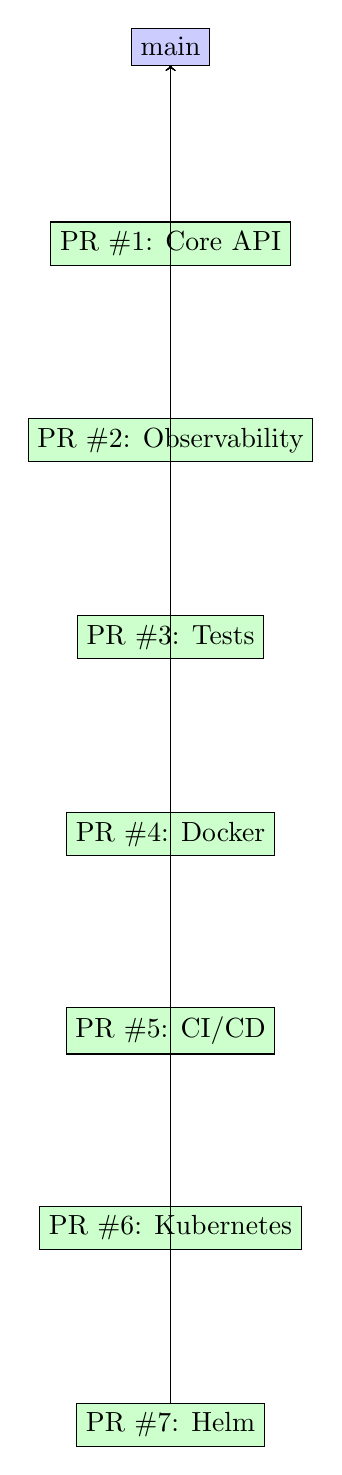
\begin{tikzpicture}[node distance=2.5cm]
    
    \node[draw, fill=blue!20] (main) {main};
    \node[draw, fill=green!20, below of=main] (pr1) {PR \#1: Core API};
    \node[draw, fill=green!20, below of=pr1] (pr2) {PR \#2: Observability};
    \node[draw, fill=green!20, below of=pr2] (pr3) {PR \#3: Tests};
    \node[draw, fill=green!20, below of=pr3] (pr4) {PR \#4: Docker};
    \node[draw, fill=green!20, below of=pr4] (pr5) {PR \#5: CI/CD};
    \node[draw, fill=green!20, below of=pr5] (pr6) {PR \#6: Kubernetes};
    \node[draw, fill=green!20, below of=pr6] (pr7) {PR \#7: Helm};
    
    \draw[<-] (main) -- (pr1);
    \draw[<-] (main) -- (pr2);
    \draw[<-] (main) -- (pr3);
    \draw[<-] (main) -- (pr4);
    \draw[<-] (main) -- (pr5);
    \draw[<-] (main) -- (pr6);
    \draw[<-] (main) -- (pr7);
    
\end{tikzpicture}
\caption{Pull Request Strategy: Contextual PRs with Single Concerns}
\end{figure}

\section{Pull Requests}

\begin{table}[h]
\centering
\begin{tabular}{|p{1.5cm}|p{4cm}|p{2cm}|}
\hline
\textbf{PR} & \textbf{Feature} & \textbf{Files} \\
\hline
\#1 & Core API Endpoints (6 endpoints) & app/main.py \\
\hline
\#2 & Observability (Prometheus + logging) & app/main.py \\
\hline
\#3 & Unit Tests (14 tests) & tests/test\_api.py \\
\hline
\#4 & Docker Containerization & Dockerfile, docker-compose.yml \\
\hline
\#5 & GitHub Actions CI/CD & .github/workflows/ci.yml \\
\hline
\#6 & Kubernetes Manifests & k8s/*.yaml \\
\hline
\#7 & Helm Charts & helm/card-signal-board/* \\
\hline
\end{tabular}
\end{table}

\chapter{Code Quality \& Testing}

\section{Unit Testing}

The project includes 14 comprehensive unit tests organized in 5 test classes:

\begin{table}[h]
\centering
\begin{tabular}{|p{3cm}|p{2cm}|p{3cm}|}
\hline
\textbf{Test Class} & \textbf{Count} & \textbf{Tests} \\
\hline
TestCardCreation & 3 & Create success, invalid email, missing fields \\
\hline
TestCardRetrieval & 4 & Empty list, with data, get success, not found \\
\hline
TestCardDeletion & 3 & Delete success, invalid token, not found \\
\hline
TestTokenVerification & 2 & Valid token, invalid token \\
\hline
TestObservability & 2 & Metrics endpoint, health check \\
\hline
\end{tabular}
\end{table}

All tests pass with 100\% endpoint coverage.

\section{Code Quality Tools}

\begin{itemize}
    \item \textbf{Black:} Code formatting (style consistency)
    \item \textbf{flake8:} Linting (code quality rules)
    \item \textbf{Bandit:} Static security analysis (security issues)
    \item \textbf{Trivy:} Container image vulnerability scanning
\end{itemize}

\chapter{Observability}

\section{Metrics Collection}

The application exposes Prometheus metrics at \texttt{/metrics} endpoint:

\begin{lstlisting}[language=python]
REQUEST_COUNT = Counter(
    'api_requests_total',
    'Total API requests',
    ['method', 'endpoint', 'status']
)

RESPONSE_TIME = Histogram(
    'api_response_time_seconds',
    'API response time in seconds',
    ['method', 'endpoint']
)
\end{lstlisting}

\section{Structured Logging}

All requests are logged with:
\begin{itemize}
    \item \textbf{Unique Request ID:} 8-character identifier for tracing
    \item \textbf{Timestamp:} ISO format with milliseconds
    \item \textbf{Method \& Path:} HTTP method and endpoint
    \item \textbf{Status Code:} Response status
    \item \textbf{Response Time:} Latency in milliseconds
\end{itemize}

\section{Health Checks}

\begin{lstlisting}[language=bash]
# Liveness Probe (every 10s)
GET /health
Response: {"status": "healthy"}

# Readiness Probe (every 5s)
GET /health
Response: {"status": "healthy"}
\end{lstlisting}

Both probes ensure pods are healthy and ready to receive traffic.

\chapter{DevOps Concepts Demonstrated}

\section{Infrastructure as Code (IaC)}

\begin{itemize}
    \item Kubernetes manifests in YAML format
    \item Helm charts for parameterized deployments
    \item Docker multi-stage builds
    \item Version-controlled infrastructure definitions
\end{itemize}

\section{Continuous Integration (CI)}

\begin{itemize}
    \item Automated testing on every push and PR
    \item Code quality checks (Black, flake8)
    \item Security scanning (Bandit, Trivy)
    \item Coverage reporting
\end{itemize}

\section{Continuous Deployment (CD)}

\begin{itemize}
    \item Automated Docker image builds
    \item Docker image vulnerability scanning
    \item Kubernetes deployment ready for manual or automated deployment
\end{itemize}

\section{Containerization}

\begin{itemize}
    \item Multi-stage Docker builds for optimization
    \item Health checks in containers
    \item Resource limits and requests
    \item Security context (non-root user, read-only filesystem)
\end{itemize}

\section{Orchestration}

\begin{itemize}
    \item Kubernetes deployment with 3 replicas
    \item Rolling updates for zero-downtime deployments
    \item Horizontal Pod Autoscaler for dynamic scaling
    \item Health probes for intelligent pod management
\end{itemize}

\section{Observability}

\begin{itemize}
    \item Prometheus metrics for monitoring
    \item Structured logging with request tracing
    \item Health endpoints for availability monitoring
    \item Graceful shutdown handling
\end{itemize}

\section{Professional Git Workflow}

\begin{itemize}
    \item Feature branches for isolated development
    \item Contextual pull requests with single concerns
    \item Code review readiness
    \item Clean commit history
    \item Merge verification
\end{itemize}

\chapter{Deployment Scenarios}

\section{Development Environment}

\begin{lstlisting}[language=bash]
# Using Helm
helm install csb ./helm/card-signal-board \
  --set replicaCount=1 \
  --set autoscaling.enabled=false \
  --set service.type=ClusterIP \
  -n development --create-namespace

# Using Docker Compose (local)
docker-compose up --build
\end{lstlisting}

\section{Staging Environment}

\begin{lstlisting}[language=bash]
helm install csb ./helm/card-signal-board \
  --set replicaCount=3 \
  --set autoscaling.minReplicas=2 \
  --set autoscaling.maxReplicas=10 \
  -n staging --create-namespace
\end{lstlisting}

\section{Production Environment}

\begin{lstlisting}[language=bash]
helm install csb ./helm/card-signal-board \
  --set replicaCount=5 \
  --set autoscaling.minReplicas=5 \
  --set autoscaling.maxReplicas=20 \
  --set resources.limits.cpu=1000m \
  --set resources.limits.memory=512Mi \
  --set image.repository=registry.azurecr.io/card-signal-board \
  --set image.tag=v1.0.0 \
  -n production --create-namespace
\end{lstlisting}

\chapter{Key Learnings}

\section{Technical Skills Acquired}

\begin{enumerate}
    \item \textbf{FastAPI Development:} Building modern REST APIs with automatic documentation
    \item \textbf{Docker:} Multi-stage builds, layer optimization, and container security
    \item \textbf{Kubernetes:} Deployments, services, health checks, auto-scaling
    \item \textbf{Helm:} Parameterized deployments and configuration management
    \item \textbf{CI/CD:} GitHub Actions workflow design and automation
    \item \textbf{Testing:} Unit testing with pytest and coverage analysis
    \item \textbf{Security:} SAST, vulnerability scanning, security context
    \item \textbf{Observability:} Metrics, logging, health checks, and monitoring
\end{enumerate}

\section{Professional Practices}

\begin{enumerate}
    \item \textbf{Version Control:} Feature branches, pull requests, code review
    \item \textbf{Single Responsibility:} Each PR addresses one concern
    \item \textbf{Automation:} Minimizing manual processes with CI/CD
    \item \textbf{Documentation:} README files and inline code comments
    \item \textbf{Best Practices:} Following Kubernetes and Docker conventions
    \item \textbf{Scalability:} Designing for horizontal scaling
\end{enumerate}

\chapter{Project Statistics}

\begin{table}[h]
\centering
\begin{tabular}{|p{3cm}|p{2cm}|}
\hline
\textbf{Metric} & \textbf{Value} \\
\hline
Lines of Code (App) & 142 \\
\hline
Lines of Code (Tests) & 179 \\
\hline
Unit Tests & 14 \\
\hline
Test Coverage & 100\% (endpoints) \\
\hline
Dockerfiles & 1 \\
\hline
Kubernetes Manifests & 6 \\
\hline
Helm Templates & 7 \\
\hline
GitHub Actions Jobs & 6 \\
\hline
Pull Requests & 7 \\
\hline
Git Commits & 15+ \\
\hline
\end{tabular}
\end{table}

\chapter{Conclusion}

This project successfully demonstrates a complete DevOps workflow from application development through production-ready deployment. By implementing:

\begin{itemize}
    \item A robust REST API with proper testing and observability
    \item Containerization with security best practices
    \item Automated CI/CD pipelines with quality gates
    \item Kubernetes orchestration with high availability
    \item Infrastructure as Code with Helm for flexibility
    \item Professional Git workflow with code review
\end{itemize}

The project serves as a comprehensive learning resource for DevOps engineers and demonstrates proficiency in modern cloud-native development practices.

\section{Future Enhancements}

Potential improvements for production deployment:
\begin{itemize}
    \item Integrate with Prometheus and Grafana for monitoring dashboards
    \item Add persistent storage with StatefulSets or managed databases
    \item Implement service mesh (Istio) for advanced traffic management
    \item Add ingress controllers for advanced routing
    \item Implement GitOps with ArgoCD for declarative deployment
    \item Add API gateway for rate limiting and authentication
\end{itemize}

\appendix

\chapter{File Reference}

\section{Repository Structure}

\begin{lstlisting}[language=bash]
card-signal-board/
├── app/
│   ├── __init__.py
│   └── main.py              # FastAPI application
├── tests/
│   └── test_api.py          # Unit tests
├── k8s/                     # Kubernetes manifests
│   ├── namespace.yaml
│   ├── deployment.yaml
│   ├── service.yaml
│   ├── configmap.yaml
│   ├── hpa.yaml
│   └── README.md
├── helm/
│   └── card-signal-board/   # Helm chart
│       ├── Chart.yaml
│       ├── values.yaml
│       ├── README.md
│       └── templates/
├── .github/
│   └── workflows/
│       ├── ci.yml           # CI/CD pipeline
│       └── docker.yml       # Docker build & push
├── Dockerfile               # Application container
├── docker-compose.yml       # Local development
├── requirements.txt         # Python dependencies
├── setup.py                 # Package configuration
└── README.md               # Project documentation
\end{lstlisting}

\section{Key Endpoints}

\begin{lstlisting}[language=bash]
# Card Management
POST   /cards                # Create card
GET    /cards                # List cards
GET    /cards/{card_id}      # Get card details
DELETE /cards/{card_id}      # Delete card (requires token)

# Verification
GET    /verify?token=...     # Verify token

# Observability
GET    /metrics              # Prometheus metrics
GET    /health               # Health check
\end{lstlisting}

\end{document}
